\documentclass[12pt. a4paper]{report}
\setcounter{secnumdepth}{0} % Turn off section numeration

\usepackage[utf8]{inputenc}
\usepackage[cache=false]{minted}
\usepackage{hyperref}
\usepackage{titlesec}
\usepackage{graphicx}
\graphicspath{ {./images/} }
\usepackage[section]{placeins}
\usepackage{tikz}
\usetikzlibrary{arrows.meta}

\titleformat{\chapter}[display]
  {\normalfont\bfseries}{}{0pt}{\Huge}

\begin{document}

\begin{titlepage}
\newlength{\drop}

\drop=0.1\textheight
\vspace*{\drop}
\centering
{\LARGE Universitatea Tehnică a Moldovei}\\[2\baselineskip]
{\LARGE\sffamily Serviciul monitoring valutar}\par
\vfill
{\LARGE LUCRARE DE AN\\
\small la disciplina \\
\large BAZE DE DATE}\par
\vspace{\drop}
{\large utilizând SGBD MySQL, PHP și stack-ul front-end la alegere \\
pentru utilizarea potențială de către o agenție specializată.}\par
\vfill
{\large\bfseries Dragomir Țurcanu\\
\small MI-191}\par
\vspace*{\drop}
{\large\bfseries Chișinău 2020}\par

\end{titlepage}


\definecolor{bg}{rgb}{0.95,0.95,0.95}
\setminted{
	breaklines=true,
	breakanywhere=true,
	bgcolor=bg,
	breaksymbolleft=,
	breakanywheresymbolpre=
}

\tableofcontents

\chapter{Conceptul SGBD}

\section{Definiția SGBD}
\textbf{SGBD} deabreviat sună ca \emph{\textbf{S}istemă de \textbf{G}estiune a \textbf{B}azelor de \textbf{D}ate}. Aceasta este o bază de date digitală bazată pe modelul relațional de date, propusă de către E.F. Codd\footnote{\url{https://en.wikipedia.org/wiki/Edgar_F._Codd}} în 1970. Sistemă softwre folosită la menținerea bazelor de date relaționale este un \textbf{SGBD}. Majoritatea sistemelor bazelor de date relaționale folosesc pentru comunicarea internă, interogări și modificări, limbajul \emph{\textbf{SQL}} \footnote{\url{https://en.wikipedia.org/wiki/SQL}}.

\section{Baze de date relaționale}
O bază de date relaționale se referă la o bază de date ce conține informația salvată într-un mod structurat, folosind \emph{randuri} și \emph{coloane}. Astfel devine simplă localizarea și accesul valorilor în cadrul bazei de date. Este numită \emph{"relațională"} deoarece valorile în fiecare \emph{\textbf{tabel}} sunt inter-conectate. Tabelele pot la fel fi conectate către alte tabele. Structura relațională creează posibilitatea de a executa \emph{\textbf{operații}} asupra a o multitudine de tabele în același moment.

\begin{figure}
\center
\includegraphics[width=\textwidth]{relational_databases_demo}
\end{figure}

\section{SGBD în practică}
SGBD-urile sunt folosite foarte intensiv în practica de zi cu zi atât a dezvoltatorilor soluțiilor software, atât și de către personalul \emph{data entry}, unitățile de management ale organizației, sau chiar \emph{stakeholder-ii} companiei. Majoritatea sistemelor moderne permit accesarea și vizualizarea datelor în format ușor accesibilă, cu funționalități performante de exportare pentru eventuală analitică folosind instrumente dezvoltate pentru însărcinarea propusă. 

Datele pot fi exportate în o multitudine bogată de formate pentru operațiuni diferite cu datele propuse. Exemple exacte sunt ce urmează.
\begin{itemize}
	\item  \emph{\textbf{JSON}}\footnote{\url{https://en.wikipedia.org/wiki/JSON}} pentru includerea în aplicații web sau scripturi, perfect pentru dezvoltatorii de soluții softare, ce au nevoie de un format portabil pentru integrarea datelor în \emph{\textbf{API}}-uri\footnote{\url{https://en.wikipedia.org/wiki/API}} și interfețe vizuale. 
	
	\item \emph{\textbf{XLS}}\footnote{\url{https://en.wikipedia.org/wiki/Microsoft_Excel}}, pentru includerea în aplicații de tip \emph{spreadsheet}, de tip Microsoft Excel, sau Google Sheets. 
	Este perfect potrivit pentru managerii sau contabilii unei companii pentru analiza și prognozartea informației pe baza datelor existente.
	
	\item \emph{\textbf{CSV}}\footnote{\url{https://en.wikipedia.org/wiki/Comma-separated_values}}, perfect pentru integrarea în scripturi și sisteme automatizate, de tipul instrumentariului pentru \emph{machine learning}\footnote{\url{https://en.wikipedia.org/wiki/Machine_learning}}. Este formatul perfect pentru experții domeniului \emph{data science} ce conlucrează cu dezvoltatorii pentru determinarea \textbf{pattern}-urilor în date, și prin urmare exploatarea parametrilor datelor pentru maximizarea profitabilității.
\end{itemize}

Cele mai răspândite sisteme de SGBD la momentul actual sunt următoarele.
\begin{itemize}
	\item Oracle DB
	\item MySQL
	\item PostreSQL
	\item SQLite
	\item Microsoft SQL Server
	\item IBM DB2
\end{itemize}

Ultimii ani, tot mai populare au inceput să devină SGBD bazate pe baze de date non-relaționale, așa numitul \emph{\textbf{NoSQL}}\footnote{\url{https://en.wikipedia.org/wiki/NoSQL}}. Acestea permit un nivel de flexibilitate a datelor mult mai înalt. Faptul dat este motivat prin lipsa unei structuri bine definite, ce prin folosirea sistemei \emph{\textbf{cheie-valoare}}.

Lipsa structurii induce o pierdere în performanță, condiționată prin complexititate indexării datelor, dar, beneficiul de bază este posibilitatea modificării formatării, mărimii sau a encodării datelor, \emph{\textbf{"on the fly"}}\footnote{În mișcare}, ce este foarte benefic pentru o sistemă software în creștere. De aia acest tip de baze de date a devenit foarte popular în cadrul \emph{\textbf{startup}}-urilor, deoarece această alegere tehnică le permite avansarea rapidă și modificarea datelor fără riscul de a strica datele.

Exemple ale astfel de SGBD sunt următoarele.
\begin{itemize}
	\item MongoDB
	\item Redis
	\item Amazon DynamoDB
	\item Oracle NoSQL DB
\end{itemize}

\chapter{Modelarea Datelor}

\section{Domeniul de studiu}

Un concept bine cunoscut oricărui investor, economist profesional, ba și unei persoane de rând, este următorul fapt: banii, bine-investiți aduc profit. Prin urmare, o persoană co-interesată, este întâlnită cu o multitudine de opțiuni pentru a o obține rezultatul dorit. În joc apar investițiile imobiliare, hârtii de preț, obiecte de epocă, dar ce-a mai răspândit în spațiul R.M., este cu siguranță inveția în valută. Diversificarea portfoliului valutar, aduce o încredere în viitorul apropiat și chiar îndelungat, fiind amplificat pe spațiul CSI de către pierderile usturătoare din anii 90'.

\emph{Ca și orice serviciu bazat pe cantitatea și calitatea datelor, alegerea valutei, monitorizarea momentului optimal de cumpărare și vânzare și calcularea tendenței de creștere și scădere a valutei este o necesitate vitală pentru orice \textbf{investor valutar}.}

Exact pentru acest scop a fost luată decizia să se creeze un sistem ușor-accesibil, bazat pe o interfață reactivă, ce ar permite o interacțiune cu fricție minimală, pentru a îndruma utilizatorii să colecteze toată informația necesară în timpul minimal, luând în considerare ritmul \textbf{supra-accelerat} a vieții cotidiene.

\section{Modelul Logic}

\begin{center}
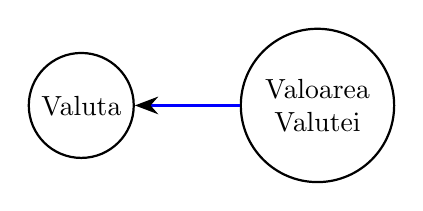
\begin{tikzpicture}
\begin{scope}[every node/.style={circle,thick,draw}]
    \node (currency) at (6,4) {Valuta};
	\node[text width=1.5cm, align=center] (currency_value) at (9, 4) {Valoarea Valutei};

\end{scope}

\begin{scope}[>={Stealth[black]},
              every node/.style={fill=white,circle},
              every edge/.style={draw=blue,very thick}]
    \path [->] (currency_value) edge (currency);

    	
\end{scope}
\end{tikzpicture}
\end{center}


Probabil modelul logic al aplicației curente pare foarte simplistic, dar secretul în cazul dat este faptul, ca acesta își îndeplinește misiunea într-un mod rapid și pragmatic. În continuare prezint machetul bazei de date.

\begin{figure}[H]
\center
\includegraphics[width=\textwidth]{currency_tracker}
\end{figure}

În cazul dat, toată structura aplicației presupune 2 tabele, \textbf{currency} și \textbf{currency\_value}, primul ce conține datele despre valutele disponibile, și al doilea tabel respectiv, despre valorile fiecărei valute într-un moment anumit de timp.

Este aplicată relația \emph{\textbf{One-To-Many}} în referință cu \textbf{currency.id}, ce este \emph{primary key} și \textbf{currency\_value.currency\_id} ce este \emph{foreign key}.

\chapter{Aspecte Tehnice}

\section{Stack-ul Tehnologic}
\begin{itemize}
	\item PHP 7.4
	\item MySQL 5.6
	\item Slim Framework \footnote{\url{https://www.slimframework.com/}}
	\item Doctrine ORM \footnote{\url{https://www.doctrine-project.org/projects/orm.html}}
	\item Git \footnote{\url{https://git-scm.com/}}
\end{itemize}

Apropos de Git, proiectul este disponibil deschis pe pagina mea proprie GitHub, pentru citire integrală și instrucțiuni de instalare. Accesați \href{https://github.com/dragomirt/lab6tw}{aici}, sau pe url-ul \url{https://github.com/dragomirt/lab6tw}.

\section{Concepția}
Ideea aplicației este crearea unei interfețe interactive pentru vizualizarea informației. Deoarece caracterul acestei informații este 
\emph{dinamic}, este logică folosirea tehnologiei \textbf{AJAX} \footnote{Asynchronous Javascript and XML}. 

Ținând acest fapt în considerare, am creat o singur loc de intrare, fișierul \textbf{index.html}, ce și conține toată partea vizuală, informația fiind încărcată prin requesturile \textbf{fetch} realizate de către client, pentru a trage informația din \textbf{endpointur-ile} ale \textbf{API-ului} \footnote{Application Programming Interface} intern.

Supranumitul API conține adrese pentru inserarea, modificarea, selectarea și ștergerea informației.

\section{Front End}
Așa deci, odată ce am discutat teoria, este timpul de a demonstra un pic de practică \emph{as well}. Mai jos este demonstrată aplicația în starea sa normală, pe unica pagină grafică a websiteului :D

\begin{figure}[H]
\centering
	\includegraphics[width=1.0\textwidth]{homepage}
\end{figure}

Pe această pagină putem admira locul primar de interacțiune a unui utilizator de rând cu aplicația în cauză. Aici este posibilă monitorizarea și selectarea valorilor pentru citire.

Majoritatea requesturilor sunt transmise de către Javascriptul din browser în formatul următor.


\begin{minted}{javascript}
    async function getCurrencyData() {
        let response = await fetch("/api/currency");
        return await response.json();
    }
\end{minted}

Fiecare request fiind modificat pentru endpoint-ul dorit. Deci requestul de sus întoarce informații generale despre toate valutele.

Funcția întreagă ce conține requestul arată în modul următor.
\begin{minted}{javascript}
    function getAvailableCurrencies() {
        let currencySelect = document.querySelector('select#currencySelect');
        let currencySelectGraph = document.querySelector('select#currencySelectGraph');

        if (!currencySelect || !currencySelectGraph) {
            return;
        }

        currencySelect.innerHTML = "";
        currencySelectGraph.innerHTML = "";

        getCurrencyData().then(data => {
            for (const row of data) {
                availableCurrencies[row.id] = {full_name: row.full_name, symbol: row.symbol};
                currencySelect.innerHTML += `<option value="${row.id}">${row.full_name}</option>`;
                currencySelectGraph.innerHTML += `<option value="${row.id}">${row.full_name}</option>`;
            }
        });
    }
\end{minted}

Aceasta ia răspunsul requestului în format \textbf{JSON} și înscrie în pagină. La fel sunt realizate celelalte blocuri din pagină.

\section{Back End}
Cum deja am menționat, alegerea a căzut pe \textbf{Slim Framework}. Aceasta a permis crearea rapidă a rutelor pentru API și descrierea simplă a logicii aplicației.

Spre exemplu, ruta ce întoarce datele despre valori, arată în modul următor.

\begin{minted}{php}
<?php
// Get all values
    $group->get('/currency/value', function(Request $request, Response $response) use (&$entityManager) { // Este funcția părinte ce encapsulează o funcție anonimă ce preia entityManager pentru a modifica datele cu ajutorul ORM
   
        $values = $entityManager->getRepository(CurrencyValue::class)->findBy([], ['created_at' => 'DESC']); // Sunt datele provenite din DB
        if ($values === null) { // Dacă valorile sunt nule, sfarsește funcția și întoarce un array gol ca http răspuns
            $response->getBody()->write(json_encode([]));
            return $response;
        }

        $responseFormatted = array();
        foreach ($values as $value) { // Pentru fiecare înscriere în DB, scrie datele în array-ul decodat pentru răspuns
            $responseFormatted[$value->getCurrency()->getId()][] = array(
                'value' => $value->getValue(),
                'date' => $value->getCreatedAt()
            );
        }

// Codifică răspunsul în format JSON și întoarce clientului
        $response->getBody()->write(json_encode($responseFormatted));
        return $response;
    });
?>
\end{minted}

Mai multe detalii sunt disponibile pe pagina GitHub a proiectului disponibilă mai sus.

\section{Adminstrare}
Pentru a permite independența managementului aplicației de la accesul direct către \textbf{SGBD}, au fost create un număr de endpointuri ale aplicației care pot fi accesate doar folosind accesul prin combinația \emph{\textbf{login + pass}}, indicată în headerul requestul spre API. Toate requesturile spre operații Create / Update / Delete sunt filtrare prin intermediul \emph{\textbf{middleware}}-ului "AdminMiddleware", ce acceptă sau revocă requestul din considerentul existenței și coincidenței headerului de authenticare cu loginul și parola de control. Astfel această aplicație exemplu primește un mic boost de securitate.

Pentru a accesa pagina de administrare, este nevoie de a naviga spre \url{/admin}. Odată încărcată, pagina va întâlni utilizatorul cu un \textbf{popup} ce va interoga utilizatorul în privința credențialelor de acces.

\begin{figure}[H]
\centering
	\includegraphics[width=1.0\textwidth]{login_popup}
\end{figure}

După inserarea datelor în interogări, administratorul este întâlnit cu următoarea interfață. Aceasta este în practică pagina de start a aplicației, cu o serie de moficiări pentru adăgurea  și modificarea datelor cu ușurință.

\begin{figure}[H]
\centering
	\includegraphics[width=1.0\textwidth]{admin_page}
\end{figure}

Astfel apar butoanele de tip \textbf{"adaugă"}, \textbf{"edit"} și \textbf{X (șterge)}. Administrarea datelor în așa caz devine foarte rapidă și luând în considerare că aici se păstrează arhitectura bazată pe \textbf{AJAX}, toată interfața este foarte interactivă și nu necesită refresh pentru a privi cele mai noi date. Pentru mai multe detalii accesați arhiva atașată sau pagina GitHub cu progresul dezvoltării lucrarii \href{https://github.com/dragomirt/lab6tw}{aici}, sau pe url-ul \url{https://github.com/dragomirt/lab6tw}.


\chapter{Concluzie}
Fiind personal interesat în domeniul investițiilor am fost fascinat să dezvolt această soluție software ce ar permite unui număr larg de persoane să-și securizeze acumulările într-un mod sigur și rapid. Pentru potențialii proprietari aplicația oferă o interfață simplă, structură BD intuitivă și cerințe către perfomanța serverului minime. Acest studiu de caz a mi-a fost o experiență deosebită de a învăța cât din plan tehnic atât și socio-profesional, având de a comunica cu un număr larg de persoane ce profită din accesul și analiza acestor date.

\end{document}
